\documentclass[11pt,a4paper]{article}
\usepackage[margin=2.5cm]{geometry}
\usepackage{amsmath,amssymb,physics}
\usepackage{tikz,tikz-3dplot}
\usepackage{pgfplots}
\pgfplotsset{compat=1.18}
\usetikzlibrary{arrows.meta,calc,decorations.pathreplacing}
\usepackage{caption,subcaption}
\usepackage[hidelinks]{hyperref}
\usepackage{xcolor}

\definecolor{ringpink}{RGB}{230,120,220}
\definecolor{axisblue}{RGB}{40,90,200}
\definecolor{planered}{RGB}{200,50,50}

\newcommand{\ke}{k_e}

\title{The Electric Potential and Field of a Uniformly Charged Ring\\ and Spherical Shell:\\
\large Why Equal Potentials Do Not Imply Equal Fields}
\author{Claude Opus 5.5}
\date{September 29, 2026}

\begin{document}
\maketitle

\begin{abstract}
The electric potential at the center of a uniformly charged ring of radius $R$ and total charge $q$ equals the potential at distance $R$ from a point charge $q$. The electric fields at these two points, however, are completely different. We explain why a single value of the potential carries no information about the field. We then compute the potential and field of the ring along its symmetry axis and in its plane, in closed form using complete elliptic integrals where necessary. Finally, we show that the center of the ring is a saddle point of the potential and discuss the consequences for the stability of a test charge, including Earnshaw's theorem. We close by contrasting the ring with a spherical shell of the same charge and radius, whose potential is constant throughout its interior.
\end{abstract}

\paragraph{Origin of this note.} This note was inspired by a sudden realization of the lecturer, Sang Hoon Lee, during his general physics lecture: the potential at the center of a uniformly charged ring has exactly the same value as the potential at distance $R$ from a point charge of the same total charge. Shortly after the lecture came the second realization, which motivates most of what follows: this equality of values alone does not provide enough information to derive the electric field of the ring.

\medskip
Throughout, $\ke \equiv 1/4\pi\varepsilon_0$, the ring lies in the $xy$-plane centered at the origin, $\rho=\sqrt{x^2+y^2}$ is the cylindrical radius, and $z$ is the coordinate along the symmetry axis.

%=====================================================================
\section{The observation: equal potentials}
%=====================================================================

The potential of a point charge $q$ at distance $R$ is
\begin{equation}
V_{\text{point}} = \frac{\ke q}{R}.
\end{equation}
For a continuous charge distribution, the potential is the scalar superposition
\begin{equation}
V(\vb r) = \ke \int \frac{dq'}{\abs{\vb r - \vb r'}}.
\label{eq:superposition}
\end{equation}
At the center of the ring, every element $dq'$ sits at the same distance $R$, so the denominator factors out:
\begin{equation}
V_{\text{ring}}(0) = \frac{\ke}{R}\int dq' = \frac{\ke q}{R} = V_{\text{point}}.
\end{equation}

\begin{figure}[h]
\centering
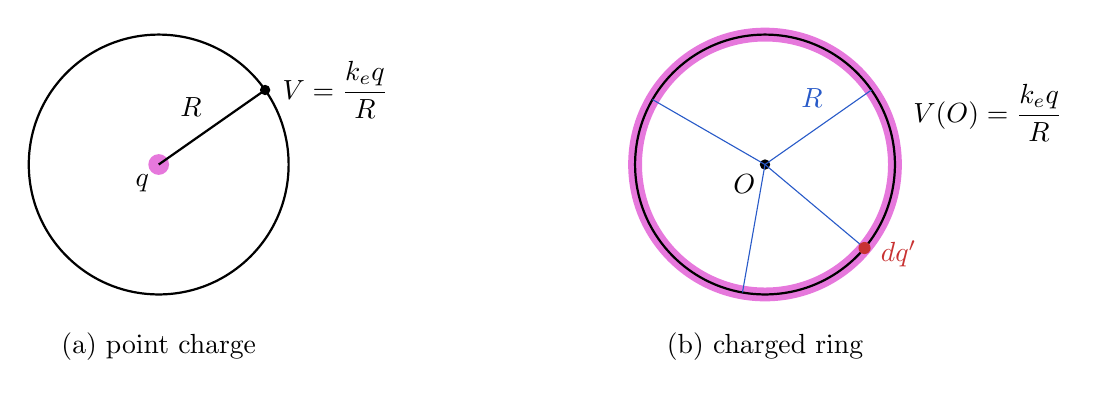
\begin{tikzpicture}[scale=1.1]
  % point charge
  \begin{scope}
    \draw[thick] (0,0) circle (1.5);
    \fill[ringpink] (0,0) circle (0.12);
    \node[below left] at (0,0) {$q$};
    \draw[thick] (0,0) -- (35:1.5) node[midway,above left] {$R$};
    \fill (35:1.5) circle (0.06);
    \node[right] at (35:1.5) {$\;V=\dfrac{\ke q}{R}$};
    \node at (0,-2.1) {(a) point charge};
  \end{scope}
  % ring
  \begin{scope}[xshift=7cm]
    \draw[ringpink,line width=5pt] (0,0) circle (1.5);
    \draw[thick] (0,0) circle (1.5);
    \fill (0,0) circle (0.06) node[below left] {$O$};
    \foreach \a in {35,150,260,320}{
      \draw[axisblue] (0,0) -- (\a:1.5);
    }
    \node[axisblue] at (35:0.95) [above left] {$R$};
    \fill[planered] (320:1.5) circle (0.07);
    \node[planered,right] at (320:1.6) {$dq'$};
    \node[right] at (1.6,0.6) {$V(O)=\dfrac{\ke q}{R}$};
    \node at (0,-2.1) {(b) charged ring};
  \end{scope}
\end{tikzpicture}
\caption{(a) The potential at distance $R$ from a point charge. (b) The potential at the center of a ring of radius $R$. Every charge element is equidistant from $O$, so the two potentials coincide.}
\label{fig:compare}
\end{figure}

The equality does not depend on the ring being a ring. \emph{Any} distribution of total charge $q$ whose every element lies at distance $R$ from the observation point produces the same potential there, including a spherical shell seen from its center.

%=====================================================================
\section{Why this does not determine the field}
%=====================================================================

The field is the negative gradient of the potential,
\begin{equation}
\vb E = -\grad V .
\end{equation}
A gradient describes how $V$ changes in a neighborhood of a point, so a single value $V(\vb r_0)$ contains no information about $\vb E(\vb r_0)$. Two functions can agree at a point and have arbitrarily different derivatives there. In the present case,
\begin{equation}
\abs{\vb E_{\text{point}}} = \frac{\ke q}{R^2},
\qquad
\vb E_{\text{ring}}(0) = \vb 0 .
\end{equation}
The second result follows at once from symmetry: contributions from diametrically opposite elements cancel pairwise. The real content lies in how $V$ and $\vb E$ \emph{vary} away from the center, which we compute next.

%=====================================================================
\section{Geometry}
%=====================================================================

\begin{figure}[h]
\centering
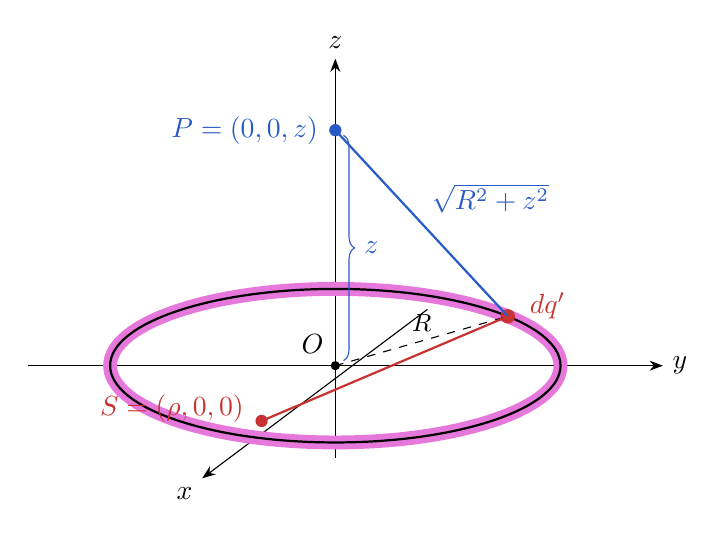
\begin{tikzpicture}[scale=1.3]
  % axes (oblique projection)
  \draw[-{Stealth}] (0,-0.9) -- (0,3.0) node[above] {$z$};
  \draw[-{Stealth}] (-3.0,0) -- (3.2,0) node[right] {$y$};
  \draw[-{Stealth}] (0.9,0.55) -- (-1.3,-1.1) node[below left] {$x$};
  % ring
  \draw[ringpink,line width=5pt] (0,0) ellipse (2.2 and 0.75);
  \draw[thick] (0,0) ellipse (2.2 and 0.75);
  \fill (0,0) circle (0.045);
  \node[above left] at (-0.02,0.02) {$O$};
  % charge element
  \coordinate (Q) at ({2.2*cos(40)},{0.75*sin(40)});
  \fill[planered] (Q) circle (0.07);
  \node[planered,right] at ($(Q)+(0.12,0.1)$) {$dq'$};
  \draw[dashed] (0,0) -- (Q) node[pos=0.5,above,font=\small] {$R$};
  % axial point P
  \coordinate (P) at (0,2.3);
  \fill[axisblue] (P) circle (0.06);
  \node[axisblue,left] at (P) {$P=(0,0,z)$\;};
  \draw[axisblue,thick] (Q) -- (P) node[midway,above right] {$\sqrt{R^2+z^2}$};
  \draw[axisblue,decorate,decoration={brace,amplitude=4pt,mirror}] (0.08,0.05) -- (0.08,2.25) node[midway,right=4pt] {$z$};
  % in-plane point S
  \coordinate (S) at (-0.72,-0.54);
  \fill[planered] (S) circle (0.06);
  \node[planered,left] at ($(S)+(-0.08,0.12)$) {$S=(\rho,0,0)$};
  \draw[planered,thick] (Q) -- (S);
\end{tikzpicture}
\caption{The ring in the $xy$-plane. From an axial point $P$ all charge elements are equidistant. From an in-plane point $S$ they are not.}
\label{fig:geometry}
\end{figure}

%=====================================================================
\section{Profile along the axis}
%=====================================================================

For $P=(0,0,z)$ every element is at distance $\sqrt{R^2+z^2}$, so Eq.~\eqref{eq:superposition} gives
\begin{equation}
V(z) = \frac{\ke q}{\sqrt{R^2+z^2}},
\qquad
E_z(z) = -\dv{V}{z} = \frac{\ke q\, z}{\left(R^2+z^2\right)^{3/2}} .
\label{eq:axis}
\end{equation}
The field vanishes at the center, grows linearly for $\abs{z}\ll R$, and reaches its maximum where $\dv*{E_z}{z}=0$:
\begin{equation}
z_{\max} = \frac{R}{\sqrt2},
\qquad
E_z^{\max} = \frac{2}{3\sqrt3}\,\frac{\ke q}{R^2}\approx 0.385\,\frac{\ke q}{R^2}.
\end{equation}
For $\abs{z}\gg R$, both expressions reduce to those of a point charge.

%=====================================================================
\section{Profile in the plane of the ring}
%=====================================================================

For $S=(\rho,0,0)$, the element at azimuth $\varphi$ is at distance $\sqrt{R^2+\rho^2-2R\rho\cos\varphi}$, which now depends on $\varphi$:
\begin{equation}
V(\rho) = \frac{\ke q}{2\pi}\int_0^{2\pi}
\frac{d\varphi}{\sqrt{R^2+\rho^2-2R\rho\cos\varphi}} .
\end{equation}
With the substitution $\varphi=\pi-2\theta$, one finds $R^2+\rho^2-2R\rho\cos\varphi=(R+\rho)^2\left(1-k^2\sin^2\theta\right)$ with modulus
\begin{equation}
k^2 = \frac{4R\rho}{(R+\rho)^2}.
\end{equation}
In terms of the complete elliptic integrals
\begin{equation}
K(k)=\int_0^{\pi/2}\frac{d\theta}{\sqrt{1-k^2\sin^2\theta}},
\qquad
E(k)=\int_0^{\pi/2}\sqrt{1-k^2\sin^2\theta}\;d\theta ,
\end{equation}
the potential and field are
\begin{align}
V(\rho) &= \frac{2\ke q}{\pi}\,\frac{K(k)}{R+\rho}, \label{eq:planeV}\\[4pt]
E_\rho(\rho) &= -\dv{V}{\rho} = \frac{\ke q}{\pi\rho\,(R+\rho)}\left[K(k)-\frac{R+\rho}{R-\rho}\,E(k)\right]. \label{eq:planeE}
\end{align}
The three regimes are as follows.
\begin{itemize}
  \item \textbf{Near the center} ($\rho\ll R$): $V\approx \dfrac{\ke q}{R}\left(1+\dfrac{\rho^2}{4R^2}\right)$ and $E_\rho\approx-\dfrac{\ke q\,\rho}{2R^3}$. The field points \emph{inward}.
  \item \textbf{Near the wire} ($\rho\to R$): $K(k)$ diverges logarithmically as $k\to1$. Locally the ring looks like an infinite line charge with $\lambda=q/2\pi R$, so
  \[
  V\sim\frac{\lambda}{2\pi\varepsilon_0}\ln\frac{8R}{\abs{R-\rho}},
  \qquad
  \abs{E_\rho}\sim\frac{\lambda}{2\pi\varepsilon_0\abs{R-\rho}} .
  \]
  The field points away from the wire on both sides.
  \item \textbf{Far away} ($\rho\gg R$): $V\to \ke q/\rho$ and $E_\rho\to \ke q/\rho^2$.
\end{itemize}

%=====================================================================
\section{Profiles compared}
%=====================================================================

In Fig.~\ref{fig:profiles}, distances are in units of $R$, potentials in units of $\ke q/R$, and fields in units of $\ke q/R^2$. The in-plane curves were computed from Eqs.~\eqref{eq:planeV}--\eqref{eq:planeE} and cross-checked against direct numerical integration of Eq.~\eqref{eq:superposition}.

\begin{figure}[h]
\centering
\begin{subfigure}{0.49\textwidth}
\centering
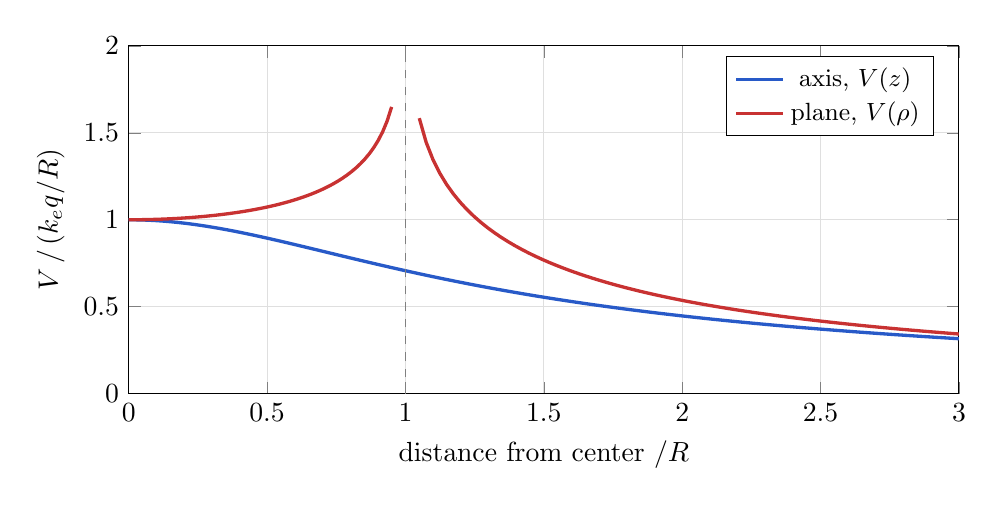
\begin{tikzpicture}
\begin{axis}[
  width=\linewidth, height=6cm,
  xlabel={distance from center $/R$},
  ylabel={$V\,/\,(\ke q/R)$},
  xmin=0, xmax=3, ymin=0, ymax=2,
  legend style={font=\small, at={(0.97,0.97)}, anchor=north east},
  grid=major, grid style={gray!25}]
  \addplot[axisblue, very thick, domain=0:3, samples=120] {1/sqrt(1+x^2)};
  \addlegendentry{axis, $V(z)$}
  \addplot[planered, very thick, forget plot] coordinates {(0.0000,1.00000) (0.0161,1.00006) (0.0322,1.00026) (0.0483,1.00058) (0.0644,1.00104) (0.0805,1.00163) (0.0966,1.00235) (0.1127,1.00320) (0.1288,1.00419) (0.1449,1.00531) (0.1610,1.00658) (0.1771,1.00798) (0.1932,1.00953) (0.2093,1.01123) (0.2254,1.01308) (0.2415,1.01508) (0.2576,1.01724) (0.2737,1.01956) (0.2898,1.02205) (0.3059,1.02472) (0.3220,1.02756) (0.3381,1.03058) (0.3542,1.03380) (0.3703,1.03721) (0.3864,1.04084) (0.4025,1.04468) (0.4186,1.04874) (0.4347,1.05305) (0.4508,1.05760) (0.4669,1.06241) (0.4831,1.06751) (0.4992,1.07289) (0.5153,1.07859) (0.5314,1.08461) (0.5475,1.09099) (0.5636,1.09774) (0.5797,1.10490) (0.5958,1.11249) (0.6119,1.12055) (0.6280,1.12912) (0.6441,1.13824) (0.6602,1.14796) (0.6763,1.15835) (0.6924,1.16946) (0.7085,1.18139) (0.7246,1.19421) (0.7407,1.20805) (0.7568,1.22303) (0.7729,1.23931) (0.7890,1.25710) (0.8051,1.27662) (0.8212,1.29819) (0.8373,1.32221) (0.8534,1.34918) (0.8695,1.37983) (0.8856,1.41514) (0.9017,1.45655) (0.9178,1.50629) (0.9339,1.56809) (0.9500,1.64885)};
  \addlegendimage{planered, very thick}
  \addlegendentry{plane, $V(\rho)$}
  \addplot[planered, very thick, forget plot] coordinates {(1.0500,1.58393) (1.0747,1.44582) (1.0994,1.34604) (1.1241,1.26765) (1.1487,1.20301) (1.1734,1.14801) (1.1981,1.10015) (1.2228,1.05781) (1.2475,1.01988) (1.2722,0.98554) (1.2968,0.95421) (1.3215,0.92542) (1.3462,0.89881) (1.3709,0.87410) (1.3956,0.85105) (1.4203,0.82947) (1.4449,0.80920) (1.4696,0.79011) (1.4943,0.77207) (1.5190,0.75499) (1.5437,0.73879) (1.5684,0.72338) (1.5930,0.70870) (1.6177,0.69470) (1.6424,0.68132) (1.6671,0.66852) (1.6918,0.65626) (1.7165,0.64450) (1.7411,0.63320) (1.7658,0.62234) (1.7905,0.61188) (1.8152,0.60181) (1.8399,0.59210) (1.8646,0.58273) (1.8892,0.57368) (1.9139,0.56494) (1.9386,0.55648) (1.9633,0.54829) (1.9880,0.54036) (2.0127,0.53268) (2.0373,0.52523) (2.0620,0.51800) (2.0867,0.51098) (2.1114,0.50416) (2.1361,0.49754) (2.1608,0.49110) (2.1854,0.48483) (2.2101,0.47874) (2.2348,0.47280) (2.2595,0.46702) (2.2842,0.46139) (2.3089,0.45590) (2.3335,0.45054) (2.3582,0.44532) (2.3829,0.44022) (2.4076,0.43524) (2.4323,0.43039) (2.4570,0.42564) (2.4816,0.42100) (2.5063,0.41647) (2.5310,0.41204) (2.5557,0.40770) (2.5804,0.40346) (2.6051,0.39932) (2.6297,0.39526) (2.6544,0.39128) (2.6791,0.38739) (2.7038,0.38357) (2.7285,0.37984) (2.7532,0.37618) (2.7778,0.37259) (2.8025,0.36907) (2.8272,0.36562) (2.8519,0.36224) (2.8766,0.35892) (2.9013,0.35566) (2.9259,0.35246) (2.9506,0.34933) (2.9753,0.34625) (3.0000,0.34322)};
  \draw[dashed, gray] (axis cs:1,0) -- (axis cs:1,2);
\end{axis}
\end{tikzpicture}
\caption{Potential}
\end{subfigure}
\hfill
\begin{subfigure}{0.49\textwidth}
\centering
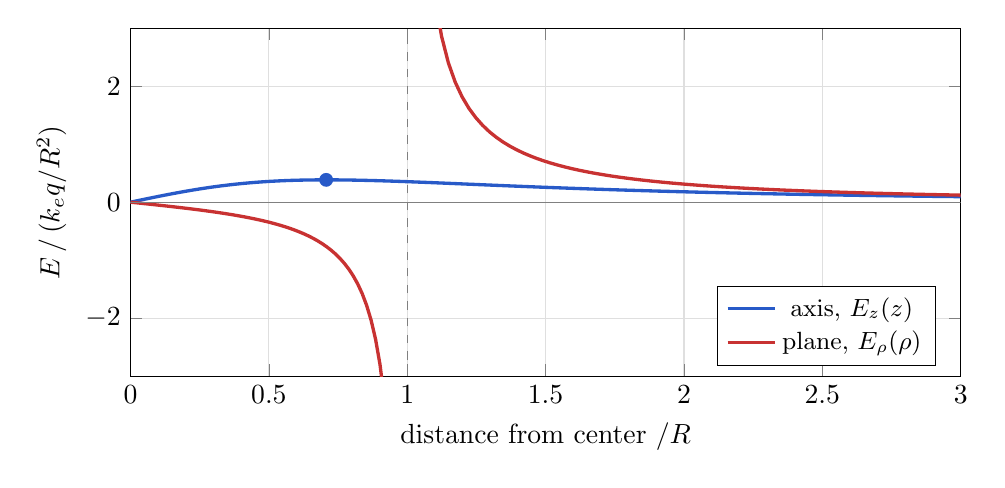
\begin{tikzpicture}
\begin{axis}[
  width=\linewidth, height=6cm,
  xlabel={distance from center $/R$},
  ylabel={$E\,/\,(\ke q/R^2)$},
  xmin=0, xmax=3, ymin=-3, ymax=3,
  restrict y to domain=-4:4,
  legend style={font=\small, at={(0.97,0.03)}, anchor=south east},
  grid=major, grid style={gray!25}]
  \addplot[axisblue, very thick, domain=0:3, samples=120] {x/(1+x^2)^1.5};
  \addlegendentry{axis, $E_z(z)$}
  \addplot[planered, very thick, forget plot] coordinates {(0.0000,0.00000) (0.0161,-0.00805) (0.0322,-0.01612) (0.0483,-0.02422) (0.0644,-0.03235) (0.0805,-0.04055) (0.0966,-0.04882) (0.1127,-0.05717) (0.1288,-0.06563) (0.1449,-0.07421) (0.1610,-0.08292) (0.1771,-0.09179) (0.1932,-0.10083) (0.2093,-0.11007) (0.2254,-0.11952) (0.2415,-0.12920) (0.2576,-0.13915) (0.2737,-0.14938) (0.2898,-0.15992) (0.3059,-0.17081) (0.3220,-0.18207) (0.3381,-0.19375) (0.3542,-0.20587) (0.3703,-0.21849) (0.3864,-0.23164) (0.4025,-0.24538) (0.4186,-0.25977) (0.4347,-0.27486) (0.4508,-0.29074) (0.4669,-0.30747) (0.4831,-0.32514) (0.4992,-0.34386) (0.5153,-0.36374) (0.5314,-0.38490) (0.5475,-0.40749) (0.5636,-0.43167) (0.5797,-0.45765) (0.5958,-0.48565) (0.6119,-0.51592) (0.6280,-0.54878) (0.6441,-0.58459) (0.6602,-0.62379) (0.6763,-0.66689) (0.6924,-0.71454) (0.7085,-0.76749) (0.7246,-0.82670) (0.7407,-0.89338) (0.7568,-0.96903) (0.7729,-1.05560) (0.7890,-1.15563) (0.8051,-1.27253) (0.8212,-1.41092) (0.8373,-1.57728) (0.8534,-1.78094) (0.8695,-2.03590) (0.8856,-2.36407) (0.9017,-2.80180) (0.9178,-3.41409) (0.9339,-4.32960) (0.9500,-5.84347)};
  \addlegendimage{planered, very thick}
  \addlegendentry{plane, $E_\rho(\rho)$}
  \addplot[planered, very thick, forget plot] coordinates {(1.0500,6.82560) (1.0747,4.64942) (1.0994,3.53888) (1.1241,2.86119) (1.1487,2.40255) (1.1734,2.07045) (1.1981,1.81823) (1.2228,1.61976) (1.2475,1.45928) (1.2722,1.32667) (1.2968,1.21514) (1.3215,1.11998) (1.3462,1.03777) (1.3709,0.96601) (1.3956,0.90281) (1.4203,0.84671) (1.4449,0.79657) (1.4696,0.75148) (1.4943,0.71072) (1.5190,0.67369) (1.5437,0.63990) (1.5684,0.60895) (1.5930,0.58050) (1.6177,0.55425) (1.6424,0.52997) (1.6671,0.50744) (1.6918,0.48649) (1.7165,0.46696) (1.7411,0.44870) (1.7658,0.43161) (1.7905,0.41558) (1.8152,0.40052) (1.8399,0.38633) (1.8646,0.37296) (1.8892,0.36033) (1.9139,0.34839) (1.9386,0.33708) (1.9633,0.32636) (1.9880,0.31618) (2.0127,0.30651) (2.0373,0.29730) (2.0620,0.28854) (2.0867,0.28019) (2.1114,0.27221) (2.1361,0.26460) (2.1608,0.25732) (2.1854,0.25036) (2.2101,0.24369) (2.2348,0.23731) (2.2595,0.23118) (2.2842,0.22530) (2.3089,0.21966) (2.3335,0.21424) (2.3582,0.20902) (2.3829,0.20401) (2.4076,0.19918) (2.4323,0.19453) (2.4570,0.19005) (2.4816,0.18573) (2.5063,0.18156) (2.5310,0.17753) (2.5557,0.17365) (2.5804,0.16989) (2.6051,0.16627) (2.6297,0.16276) (2.6544,0.15936) (2.6791,0.15608) (2.7038,0.15290) (2.7285,0.14982) (2.7532,0.14683) (2.7778,0.14394) (2.8025,0.14114) (2.8272,0.13841) (2.8519,0.13577) (2.8766,0.13321) (2.9013,0.13072) (2.9259,0.12830) (2.9506,0.12595) (2.9753,0.12367) (3.0000,0.12145)};
  \draw[dashed, gray] (axis cs:1,-3) -- (axis cs:1,3);
  \draw[gray] (axis cs:0,0) -- (axis cs:3,0);
  \fill[axisblue] (axis cs:0.7071,0.3849) circle (2.5pt);
\end{axis}
\end{tikzpicture}
\caption{Field component}
\end{subfigure}
\caption{Potential and field of the ring along the axis (blue) and in the plane (red). The dashed line marks the wire at $\rho=R$, where the in-plane quantities diverge. The dot marks the maximum of $E_z$ at $z=R/\sqrt2$.}
\label{fig:profiles}
\end{figure}

Both potentials start at $\ke q/R$ but curve in opposite directions: $V$ decreases along the axis and increases in the plane. This is the saddle structure discussed next.

%=====================================================================
\section{Local structure: a saddle point}
%=====================================================================

Combining the small-distance expansions of Eqs.~\eqref{eq:axis} and \eqref{eq:planeV},
\begin{equation}
V(\rho,z)\approx\frac{\ke q}{R}\left(1+\frac{\rho^2}{4R^2}-\frac{z^2}{2R^2}\right)
=\frac{\ke q}{R}\left(1+\frac{x^2+y^2-2z^2}{4R^2}\right).
\label{eq:local}
\end{equation}
This satisfies Laplace's equation, as it must in charge-free space:
\begin{equation}
\laplacian V \propto \underbrace{\tfrac12+\tfrac12}_{x,\,y}\;\underbrace{-\,1}_{z} = 0 .
\end{equation}
The local field is
\begin{equation}
\vb E \approx \frac{\ke q}{2R^3}\,\left(-x,\,-y,\,2z\right).
\label{eq:localE}
\end{equation}

\begin{figure}[h]
\centering
\begin{subfigure}{0.49\textwidth}
\centering
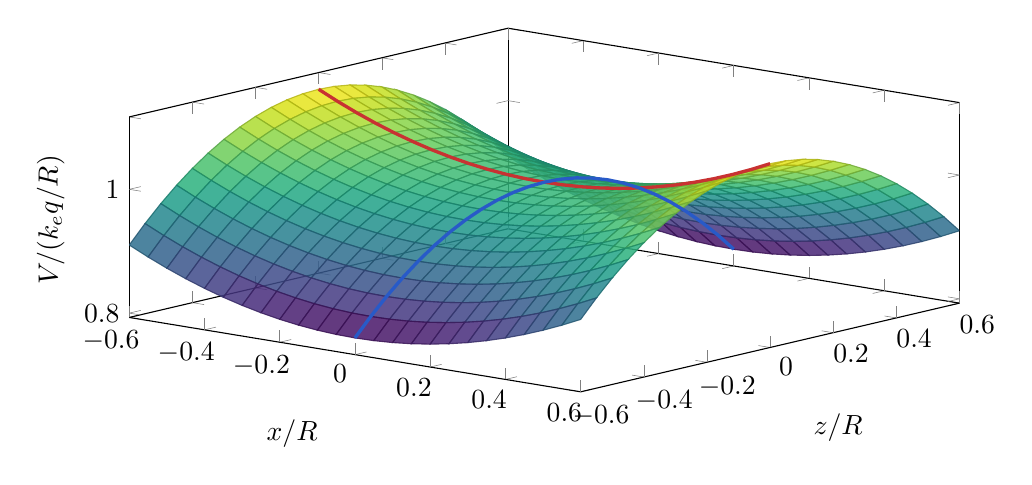
\begin{tikzpicture}
\begin{axis}[
  width=\linewidth, height=6.2cm,
  view={40}{30},
  xlabel={$x/R$}, ylabel={$z/R$},
  zlabel={$V/(\ke q/R)$},
  colormap/viridis, samples=25,
  domain=-0.6:0.6, y domain=-0.6:0.6]
  \addplot3[surf, opacity=0.85] {1 + x^2/4 - y^2/2};
  \addplot3[planered, very thick, domain=-0.6:0.6, samples y=0] (x,0,{1+x^2/4});
  \addplot3[axisblue, very thick, domain=-0.6:0.6, samples y=0] (0,x,{1-x^2/2});
\end{axis}
\end{tikzpicture}
\caption{$V$ in the $xz$-plane near $O$}
\end{subfigure}
\hfill
\begin{subfigure}{0.49\textwidth}
\centering
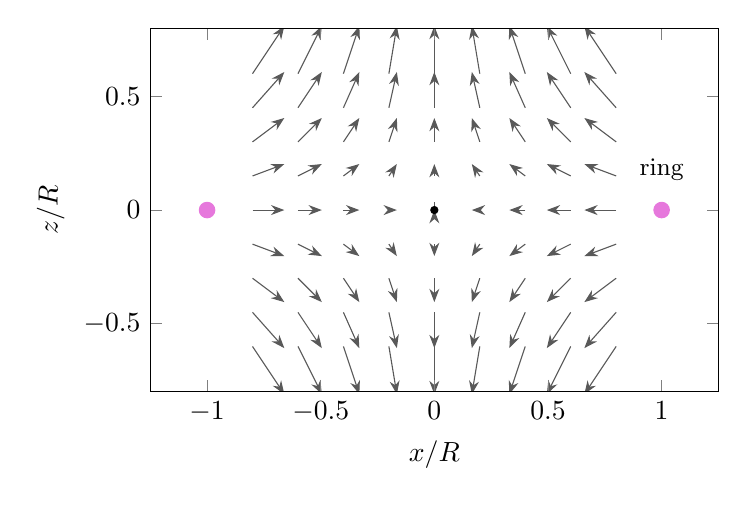
\begin{tikzpicture}
\begin{axis}[
  width=\linewidth, height=6.2cm,
  xlabel={$x/R$}, ylabel={$z/R$},
  xmin=-1.25, xmax=1.25, ymin=-0.8, ymax=0.8,
  view={0}{90}, axis equal image]
  \addplot3[
    quiver={u={-x/2}, v={y}, w=0, scale arrows=0.35},
    -{Stealth}, gray!70!black,
    samples=9, domain=-0.8:0.8, y domain=-0.6:0.6]
    (x,y,0);
  \fill[ringpink] (axis cs:-1,0) circle (3pt);
  \fill[ringpink] (axis cs:1,0) circle (3pt);
  \node[font=\small] at (axis cs:1,0.18) {ring};
  \fill (axis cs:0,0) circle (1.5pt);
\end{axis}
\end{tikzpicture}
\caption{Local field, Eq.~\eqref{eq:localE}}
\end{subfigure}
\caption{The center of the ring is a saddle point. (a) Near $O$, $V$ rises along $x$ (red) and falls along $z$ (blue). (b) The field in the $xz$ cross-section, where the ring appears as two dots at $x=\pm R$. It points toward $O$ in the plane and away from $O$ along the axis.}
\label{fig:saddle}
\end{figure}

%=====================================================================
\section{Stability of a test charge}
%=====================================================================

A test charge $Q$ has potential energy $U=QV$. Near the center,
\begin{equation}
U\approx\frac{\ke qQ}{R}\left(1+\frac{\rho^2}{4R^2}-\frac{z^2}{2R^2}\right).
\end{equation}

\paragraph{Same sign ($qQ>0$).} $U$ has a minimum in the plane and a maximum along the axis. The charge is pushed back toward $O$ within the plane but expelled along $z$.

\paragraph{Opposite sign ($qQ<0$).} The roles reverse. The charge is attracted to $O$ along the axis but pulled toward the wire by any in-plane displacement.

\paragraph{Overall instability.} An equilibrium in three dimensions is stable only if it is restoring in \emph{every} direction. A generic perturbation has a component along the unstable direction, and that component grows exponentially. The center is therefore unstable for either sign of $Q$. This is a special case of \textbf{Earnshaw's theorem}: since $\laplacian V=0$ in charge-free space, $V$ cannot have a local minimum or maximum there, so no static arrangement of charges can stably trap a charge.

\paragraph{Constrained motion.} If a constraint removes the unstable direction, the center becomes stable, and small oscillations have angular frequencies
\begin{align}
\omega_\rho^2&=\frac{\ke qQ}{2mR^3} &&(qQ>0,\ \text{motion confined to the plane}),\\
\omega_z^2&=\frac{\ke q\abs{Q}}{mR^3} &&(qQ<0,\ \text{motion confined to the axis}).
\end{align}
The relation $\omega_z^2=2\omega_\rho^2$ reflects Laplace's equation: the curvature along $z$ balances the combined curvature along $x$ and $y$.

\paragraph{Evading Earnshaw.} Practical ion traps exploit exactly this saddle geometry. A \emph{Paul trap} makes the saddle alternate its orientation with a radio-frequency voltage, producing net confinement on average. A \emph{Penning trap} keeps a static electric saddle and adds a strong axial magnetic field to confine the particle in the unstable directions.

%=====================================================================
\section{The spherical shell: the three-dimensional analogue}
%=====================================================================

Spread the same charge $q$ uniformly over a spherical shell of radius $R$ instead of a ring. The potential at the center is again $\ke q/R$, because every element is at distance $R$. Unlike the ring, however, the shell is simple enough that the complete profile follows in a few lines, and the result is far more intuitive.

\subsection{Direct integration}

Let the observation point $P$ be at distance $r$ from the center, and slice the shell into thin rings coaxial with the line $OP$, as in Fig.~\ref{fig:shell}(a). The ring at polar angle $\theta$ carries charge $dq=\tfrac{q}{2}\sin\theta\,d\theta$, and all of it is at the same distance
\begin{equation}
s^2 = R^2 + r^2 - 2Rr\cos\theta
\qquad\Longrightarrow\qquad
s\,ds = Rr\sin\theta\,d\theta .
\end{equation}
The change of variables from $\theta$ to $s$ makes the integral elementary:
\begin{equation}
V(r) = \ke\int\frac{dq}{s}
= \frac{\ke q}{2}\int_0^\pi\frac{\sin\theta\,d\theta}{s}
= \frac{\ke q}{2Rr}\int_{\abs{R-r}}^{R+r} ds
= \frac{\ke q}{2Rr}\Big[(R+r)-\abs{R-r}\Big].
\end{equation}
Hence
\begin{equation}
V(r)=
\begin{cases}
\dfrac{\ke q}{R}, & r<R,\\[10pt]
\dfrac{\ke q}{r}, & r>R,
\end{cases}
\qquad\qquad
E_r(r)=
\begin{cases}
0, & r<R,\\[6pt]
\dfrac{\ke q}{r^2}, & r>R.
\end{cases}
\label{eq:shell}
\end{equation}
Outside, the shell is indistinguishable from a point charge at its center. Inside, the potential is \emph{constant}, equal everywhere to its value at the center, and the field vanishes identically. The same results follow in one line from Gauss's law, since a spherical Gaussian surface inside the shell encloses no charge.

The slicing makes the relation to the ring explicit: \emph{the shell is a superposition of rings}. Each individual ring produces a saddle-shaped potential, but when rings are stacked over the full sphere, the curvatures cancel in every direction and the saddles flatten into a constant.

\subsection{Why the field vanishes inside: Newton's cone argument}

There is a purely geometric reason for the vanishing interior field. From an interior point $P$, draw a thin double cone of solid angle $d\Omega$, as in Fig.~\ref{fig:shell}(b). It cuts two patches from the shell, at distances $s_1$ and $s_2$. Both patches meet the cone at the same angle $\alpha$, because the chord through $P$ makes equal angles with the sphere at its two ends. Their areas are therefore $s_i^2\,d\Omega/\cos\alpha$, and their charges are
\begin{equation}
dq_i = \sigma\,\frac{s_i^2\,d\Omega}{\cos\alpha},
\qquad
\abs{d\vb E_i} = \frac{\ke\,dq_i}{s_i^2} = \frac{\ke\sigma\,d\Omega}{\cos\alpha}.
\end{equation}
The two contributions are equal in magnitude and opposite in direction. The nearer patch is closer, but it is proportionally smaller: the $s^2$ growth of area exactly compensates the $1/s^2$ decay of the Coulomb field. Pairing up all such cones gives $\vb E=\vb 0$ at every interior point, not just at the center.

The ring has no such compensation. It is a one-dimensional distribution, so the charge cut from it by a thin wedge of opening angle $d\varphi$ through $P$ grows only like $s$, not $s^2$, and the field contributions scale as $1/s$. The nearer side of the ring wins. This is why the in-plane field of the ring points \emph{away} from the nearer part of the wire, that is, back toward the center.

\begin{figure}[h]
\centering
\begin{subfigure}{0.47\textwidth}
\centering
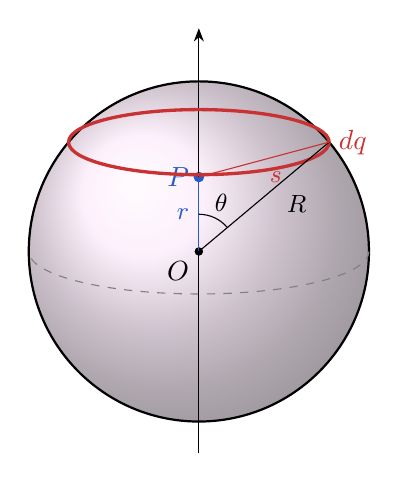
\begin{tikzpicture}[scale=1.35]
  \shade[ball color=ringpink!25, opacity=0.6] (0,0) circle (1.6);
  \draw[thick] (0,0) circle (1.6);
  \draw[dashed,gray] (1.6,0) arc (0:-180:1.6 and 0.4);
  \fill (0,0) circle (0.04) node[below left] {$O$};
  \coordinate (P) at (0,0.7);
  \fill[axisblue] (P) circle (0.05) node[left] {$P$};
  \draw[-{Stealth}] (0,-1.9) -- (0,2.1);
  \draw[axisblue] (0,0) -- (P) node[midway,left,font=\small] {$r$};
  % slicing ring at theta
  \pgfmathsetmacro{\th}{50}
  \pgfmathsetmacro{\rx}{1.6*sin(\th)}
  \pgfmathsetmacro{\zz}{1.6*cos(\th)}
  \draw[planered,very thick] (0,\zz) ellipse ({\rx} and {0.25*\rx/1.6*1.6*0.25*4});
  \coordinate (Q) at (\rx,\zz);
  \draw (0,0) -- (Q) node[pos=0.6,below right,font=\small] {$R$};
  \draw[planered] (Q) -- (P);
  \node[planered,font=\small] at ($(P)!0.55!(Q)+(0.05,-0.18)$) {$s$};
  \draw (0,0.35) arc (90:{90-\th}:0.35);
  \node[font=\small] at ({0.5*cos(90-\th/2)},{0.5*sin(90-\th/2)}) {$\theta$};
  \node[planered,right] at (Q) {$dq$};
\end{tikzpicture}
\caption{Slicing the shell into coaxial rings}
\end{subfigure}
\hfill
\begin{subfigure}{0.47\textwidth}
\centering
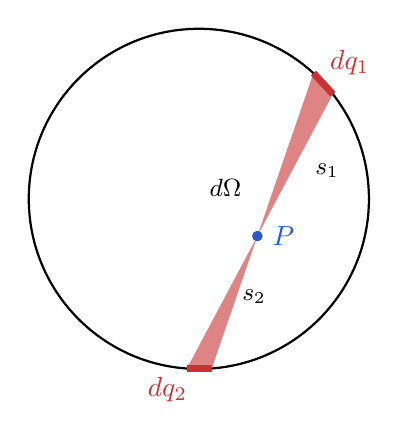
\begin{tikzpicture}[scale=1.35]
  \draw[thick] (0,0) circle (1.6);
  \coordinate (P) at (0.55,-0.35);
  % chord directions
  \pgfmathsetmacro{\phiA}{62}
  \pgfmathsetmacro{\dphi}{9}
  % intersection of ray from P with circle: solve |P + t u| = R
  \foreach \ang/\nm in {\phiA/a1,{\phiA+\dphi}/a2,{\phiA+180}/b1,{\phiA+\dphi+180}/b2}{
    \pgfmathsetmacro{\ux}{cos(\ang)}
    \pgfmathsetmacro{\uy}{sin(\ang)}
    \pgfmathsetmacro{\pu}{0.55*\ux-0.35*\uy}
    \pgfmathsetmacro{\t}{-\pu+sqrt(\pu*\pu-(0.55*0.55+0.35*0.35)+1.6*1.6)}
    \coordinate (\nm) at ({0.55+\t*\ux},{-0.35+\t*\uy});
  }
  \fill[planered!60] (P) -- (a1) -- (a2) -- cycle;
  \fill[planered!60] (P) -- (b1) -- (b2) -- cycle;
  \draw[planered,line width=2.5pt] (a1) -- (a2);
  \draw[planered,line width=2.5pt] (b1) -- (b2);
  \fill[axisblue] (P) circle (0.05) node[right=2pt] {$P$};
  \node[planered] at ($(a1)!0.5!(a2)+(0.25,0.2)$) {$dq_1$};
  \node[planered] at ($(b1)!0.5!(b2)+(-0.3,-0.2)$) {$dq_2$};
  \node[font=\small] at ($(P)!0.5!(a1)+(0.3,-0.05)$) {$s_1$};
  \node[font=\small] at ($(P)!0.5!(b1)+(0.3,0.05)$) {$s_2$};
  \node[font=\small] at ($(P)+(-0.3,0.45)$) {$d\Omega$};
\end{tikzpicture}
\caption{Newton's double-cone argument}
\end{subfigure}
\caption{(a) Every point of the shaded ring at polar angle $\theta$ is at the same distance $s$ from $P$, which reduces the shell to a one-variable integral. (b) The two patches cut by a thin double cone through an interior point have charges proportional to $s_1^2$ and $s_2^2$, so their fields cancel exactly.}
\label{fig:shell}
\end{figure}

\subsection{Profiles and comparison with the ring}

\begin{figure}[h]
\centering
\begin{subfigure}{0.49\textwidth}
\centering
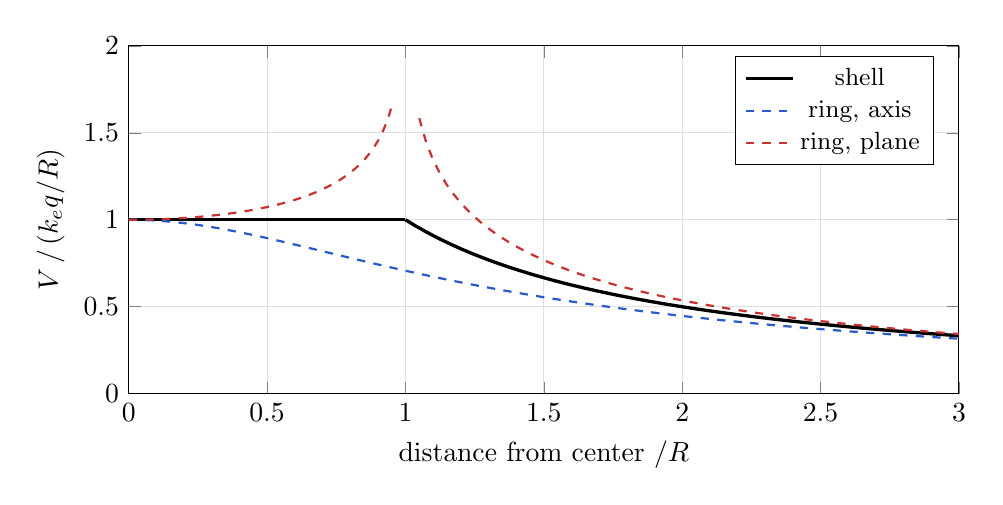
\begin{tikzpicture}
\begin{axis}[
  width=\linewidth, height=6cm,
  xlabel={distance from center $/R$},
  ylabel={$V\,/\,(\ke q/R)$},
  xmin=0, xmax=3, ymin=0, ymax=2,
  legend style={font=\small, at={(0.97,0.97)}, anchor=north east},
  grid=major, grid style={gray!25}]
  \addplot[black, very thick, domain=0:1] {1};
  \addlegendentry{shell}
  \addplot[black, very thick, domain=1:3, samples=60, forget plot] {1/x};
  \addplot[axisblue, thick, dashed, domain=0:3, samples=120] {1/sqrt(1+x^2)};
  \addlegendentry{ring, axis}
  \addplot[planered, thick, dashed, forget plot] coordinates {(0.0000,1.00000) (0.0161,1.00006) (0.0322,1.00026) (0.0483,1.00058) (0.0644,1.00104) (0.0805,1.00163) (0.0966,1.00235) (0.1127,1.00320) (0.1288,1.00419) (0.1449,1.00531) (0.1610,1.00658) (0.1771,1.00798) (0.1932,1.00953) (0.2093,1.01123) (0.2254,1.01308) (0.2415,1.01508) (0.2576,1.01724) (0.2737,1.01956) (0.2898,1.02205) (0.3059,1.02472) (0.3220,1.02756) (0.3381,1.03058) (0.3542,1.03380) (0.3703,1.03721) (0.3864,1.04084) (0.4025,1.04468) (0.4186,1.04874) (0.4347,1.05305) (0.4508,1.05760) (0.4669,1.06241) (0.4831,1.06751) (0.4992,1.07289) (0.5153,1.07859) (0.5314,1.08461) (0.5475,1.09099) (0.5636,1.09774) (0.5797,1.10490) (0.5958,1.11249) (0.6119,1.12055) (0.6280,1.12912) (0.6441,1.13824) (0.6602,1.14796) (0.6763,1.15835) (0.6924,1.16946) (0.7085,1.18139) (0.7246,1.19421) (0.7407,1.20805) (0.7568,1.22303) (0.7729,1.23931) (0.7890,1.25710) (0.8051,1.27662) (0.8212,1.29819) (0.8373,1.32221) (0.8534,1.34918) (0.8695,1.37983) (0.8856,1.41514) (0.9017,1.45655) (0.9178,1.50629) (0.9339,1.56809) (0.9500,1.64885)};
  \addlegendimage{planered, thick, dashed}
  \addlegendentry{ring, plane}
  \addplot[planered, thick, dashed, forget plot] coordinates {(1.0500,1.58393) (1.0747,1.44582) (1.0994,1.34604) (1.1241,1.26765) (1.1487,1.20301) (1.1734,1.14801) (1.1981,1.10015) (1.2228,1.05781) (1.2475,1.01988) (1.2722,0.98554) (1.2968,0.95421) (1.3215,0.92542) (1.3462,0.89881) (1.3709,0.87410) (1.3956,0.85105) (1.4203,0.82947) (1.4449,0.80920) (1.4696,0.79011) (1.4943,0.77207) (1.5190,0.75499) (1.5437,0.73879) (1.5684,0.72338) (1.5930,0.70870) (1.6177,0.69470) (1.6424,0.68132) (1.6671,0.66852) (1.6918,0.65626) (1.7165,0.64450) (1.7411,0.63320) (1.7658,0.62234) (1.7905,0.61188) (1.8152,0.60181) (1.8399,0.59210) (1.8646,0.58273) (1.8892,0.57368) (1.9139,0.56494) (1.9386,0.55648) (1.9633,0.54829) (1.9880,0.54036) (2.0127,0.53268) (2.0373,0.52523) (2.0620,0.51800) (2.0867,0.51098) (2.1114,0.50416) (2.1361,0.49754) (2.1608,0.49110) (2.1854,0.48483) (2.2101,0.47874) (2.2348,0.47280) (2.2595,0.46702) (2.2842,0.46139) (2.3089,0.45590) (2.3335,0.45054) (2.3582,0.44532) (2.3829,0.44022) (2.4076,0.43524) (2.4323,0.43039) (2.4570,0.42564) (2.4816,0.42100) (2.5063,0.41647) (2.5310,0.41204) (2.5557,0.40770) (2.5804,0.40346) (2.6051,0.39932) (2.6297,0.39526) (2.6544,0.39128) (2.6791,0.38739) (2.7038,0.38357) (2.7285,0.37984) (2.7532,0.37618) (2.7778,0.37259) (2.8025,0.36907) (2.8272,0.36562) (2.8519,0.36224) (2.8766,0.35892) (2.9013,0.35566) (2.9259,0.35246) (2.9506,0.34933) (2.9753,0.34625) (3.0000,0.34322)};
\end{axis}
\end{tikzpicture}
\caption{Potential}
\end{subfigure}
\hfill
\begin{subfigure}{0.49\textwidth}
\centering
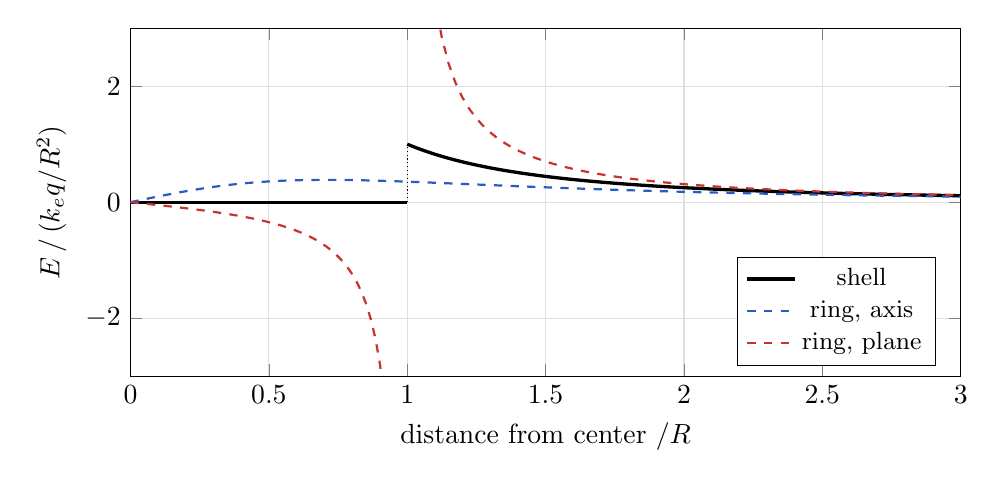
\begin{tikzpicture}
\begin{axis}[
  width=\linewidth, height=6cm,
  xlabel={distance from center $/R$},
  ylabel={$E\,/\,(\ke q/R^2)$},
  xmin=0, xmax=3, ymin=-3, ymax=3,
  restrict y to domain=-4:4,
  legend style={font=\small, at={(0.97,0.03)}, anchor=south east},
  grid=major, grid style={gray!25}]
  \addplot[black, very thick, domain=0:1] {0};
  \addlegendentry{shell}
  \addplot[black, very thick, domain=1:3, samples=60, forget plot] {1/x^2};
  \draw[black, densely dotted] (axis cs:1,0) -- (axis cs:1,1);
  \addplot[axisblue, thick, dashed, domain=0:3, samples=120] {x/(1+x^2)^1.5};
  \addlegendentry{ring, axis}
  \addplot[planered, thick, dashed, forget plot] coordinates {(0.0000,0.00000) (0.0161,-0.00805) (0.0322,-0.01612) (0.0483,-0.02422) (0.0644,-0.03235) (0.0805,-0.04055) (0.0966,-0.04882) (0.1127,-0.05717) (0.1288,-0.06563) (0.1449,-0.07421) (0.1610,-0.08292) (0.1771,-0.09179) (0.1932,-0.10083) (0.2093,-0.11007) (0.2254,-0.11952) (0.2415,-0.12920) (0.2576,-0.13915) (0.2737,-0.14938) (0.2898,-0.15992) (0.3059,-0.17081) (0.3220,-0.18207) (0.3381,-0.19375) (0.3542,-0.20587) (0.3703,-0.21849) (0.3864,-0.23164) (0.4025,-0.24538) (0.4186,-0.25977) (0.4347,-0.27486) (0.4508,-0.29074) (0.4669,-0.30747) (0.4831,-0.32514) (0.4992,-0.34386) (0.5153,-0.36374) (0.5314,-0.38490) (0.5475,-0.40749) (0.5636,-0.43167) (0.5797,-0.45765) (0.5958,-0.48565) (0.6119,-0.51592) (0.6280,-0.54878) (0.6441,-0.58459) (0.6602,-0.62379) (0.6763,-0.66689) (0.6924,-0.71454) (0.7085,-0.76749) (0.7246,-0.82670) (0.7407,-0.89338) (0.7568,-0.96903) (0.7729,-1.05560) (0.7890,-1.15563) (0.8051,-1.27253) (0.8212,-1.41092) (0.8373,-1.57728) (0.8534,-1.78094) (0.8695,-2.03590) (0.8856,-2.36407) (0.9017,-2.80180) (0.9178,-3.41409) (0.9339,-4.32960) (0.9500,-5.84347)};
  \addlegendimage{planered, thick, dashed}
  \addlegendentry{ring, plane}
  \addplot[planered, thick, dashed, forget plot] coordinates {(1.0500,6.82560) (1.0747,4.64942) (1.0994,3.53888) (1.1241,2.86119) (1.1487,2.40255) (1.1734,2.07045) (1.1981,1.81823) (1.2228,1.61976) (1.2475,1.45928) (1.2722,1.32667) (1.2968,1.21514) (1.3215,1.11998) (1.3462,1.03777) (1.3709,0.96601) (1.3956,0.90281) (1.4203,0.84671) (1.4449,0.79657) (1.4696,0.75148) (1.4943,0.71072) (1.5190,0.67369) (1.5437,0.63990) (1.5684,0.60895) (1.5930,0.58050) (1.6177,0.55425) (1.6424,0.52997) (1.6671,0.50744) (1.6918,0.48649) (1.7165,0.46696) (1.7411,0.44870) (1.7658,0.43161) (1.7905,0.41558) (1.8152,0.40052) (1.8399,0.38633) (1.8646,0.37296) (1.8892,0.36033) (1.9139,0.34839) (1.9386,0.33708) (1.9633,0.32636) (1.9880,0.31618) (2.0127,0.30651) (2.0373,0.29730) (2.0620,0.28854) (2.0867,0.28019) (2.1114,0.27221) (2.1361,0.26460) (2.1608,0.25732) (2.1854,0.25036) (2.2101,0.24369) (2.2348,0.23731) (2.2595,0.23118) (2.2842,0.22530) (2.3089,0.21966) (2.3335,0.21424) (2.3582,0.20902) (2.3829,0.20401) (2.4076,0.19918) (2.4323,0.19453) (2.4570,0.19005) (2.4816,0.18573) (2.5063,0.18156) (2.5310,0.17753) (2.5557,0.17365) (2.5804,0.16989) (2.6051,0.16627) (2.6297,0.16276) (2.6544,0.15936) (2.6791,0.15608) (2.7038,0.15290) (2.7285,0.14982) (2.7532,0.14683) (2.7778,0.14394) (2.8025,0.14114) (2.8272,0.13841) (2.8519,0.13577) (2.8766,0.13321) (2.9013,0.13072) (2.9259,0.12830) (2.9506,0.12595) (2.9753,0.12367) (3.0000,0.12145)};
\end{axis}
\end{tikzpicture}
\caption{Field}
\end{subfigure}
\caption{The shell (solid black) compared with the ring (dashed, from Fig.~\ref{fig:profiles}). The shell's potential is flat inside and continuous at $r=R$. Its field jumps from $0$ to $\ke q/R^2=\sigma/\varepsilon_0$ across the surface, the standard discontinuity for a surface charge. The ring's line charge instead produces a divergence at the wire.}
\label{fig:shellprofiles}
\end{figure}

Figure~\ref{fig:shellprofiles} and Table~\ref{tab:compare} summarize the differences. The shell's potential has no curvature inside at all, so $\laplacian V=0$ is satisfied trivially rather than through the balance of opposite curvatures seen for the ring. A test charge inside the shell feels no force anywhere: its equilibrium is \emph{neutral}, neither stable nor unstable. This is still consistent with Earnshaw's theorem, which forbids a strict minimum but not a flat potential.

\begin{table}[h]
\centering
\renewcommand{\arraystretch}{1.45}
\begin{tabular}{lcc}
\hline
 & ring (1D charge) & spherical shell (2D charge) \\
\hline
$V$ at center & $\ke q/R$ & $\ke q/R$ \\
$\vb E$ at center & $\vb 0$ & $\vb 0$ \\
$\vb E$ elsewhere inside & nonzero & $\vb 0$ everywhere \\
$V$ near center & saddle: $\dfrac{\ke q}{R}\Big(1+\dfrac{x^2+y^2-2z^2}{4R^2}\Big)$ & constant \\
behavior at the charge & $V$, $\vb E$ diverge & $V$ continuous, $\vb E$ jumps by $\sigma/\varepsilon_0$ \\
equilibrium at center & unstable (saddle) & neutral \\
closed form & elliptic integrals & elementary \\
\hline
\end{tabular}
\caption{The ring and the spherical shell of equal charge and radius.}
\label{tab:compare}
\end{table}

The shell also sharpens the lesson of Sec.~2. The shell, the ring, and the point charge at distance $R$ all give the \emph{same} potential at one point, yet their fields there are $\vb 0$, $\vb 0$, and $\ke q/R^2$, and the shell and ring differ everywhere else. A single value of $V$ says nothing about the configuration that produced it.

%=====================================================================
\section{Summary}
%=====================================================================

\begin{itemize}
  \item At a single point, $V$ depends only on the distances to the charges. This is why the ring's central potential equals that of a point charge at distance $R$.
  \item $\vb E=-\grad V$ depends on how $V$ varies near the point, so it cannot be deduced from one value of $V$. To find $\vb E$, compute $V$ at a general point, differentiate, and only then evaluate.
  \item Along the axis, $V$ and $E_z$ have elementary closed forms. In the plane, they require complete elliptic integrals.
  \item The center of the ring is a saddle point of $V$. A test charge there is in unstable equilibrium regardless of its sign, as Earnshaw's theorem requires.
  \item A spherical shell of the same charge and radius gives the same central potential, but its potential is constant throughout the interior and its field vanishes everywhere inside. Area growing as $s^2$ compensates the $1/s^2$ field exactly, a compensation that a one-dimensional ring cannot provide.
\end{itemize}

\appendix
\section{Field at a general point}
For completeness, at $(\rho,z)$ with $k^2=4R\rho/\left[(R+\rho)^2+z^2\right]$,
\begin{align}
V&=\frac{2\ke q}{\pi}\,\frac{K(k)}{\sqrt{(R+\rho)^2+z^2}},\\
E_z&=\frac{2\ke q}{\pi}\,\frac{z\,E(k)}{\left[(R-\rho)^2+z^2\right]\sqrt{(R+\rho)^2+z^2}},\\
E_\rho&=\frac{\ke q}{\pi\rho\sqrt{(R+\rho)^2+z^2}}
\left[K(k)+\frac{\rho^2-R^2-z^2}{(R-\rho)^2+z^2}\,E(k)\right].
\end{align}
Setting $\rho=0$ recovers Eq.~\eqref{eq:axis}, and setting $z=0$ recovers Eqs.~\eqref{eq:planeV}--\eqref{eq:planeE}.

\end{document}
